\chapter{Modélisation des données et Évaluation}
\epigraph{Economists and agronomists are locked in debate about likely
future yields. Since the method of the economists is to predict
future outcomes from past performance, economists expect
success to continue. And since for the scientists future success
depends on discoveries they will have to make and do not now
know how to make, the scientists are doubtful. At its core, this is
a disagreement about the pace of technical change.}{Robert
Socolow}
\cleardoublepage

	\section{Analyse causale}
	\begin{Huge}{ En cours de construction}
		\end{Huge}
	\section{Analyse en séries chronologiques et projections}
	Étude de la série "Demande en fertilisant du brésil "
	\begin{figure}[H]
		\centering
		\fbox{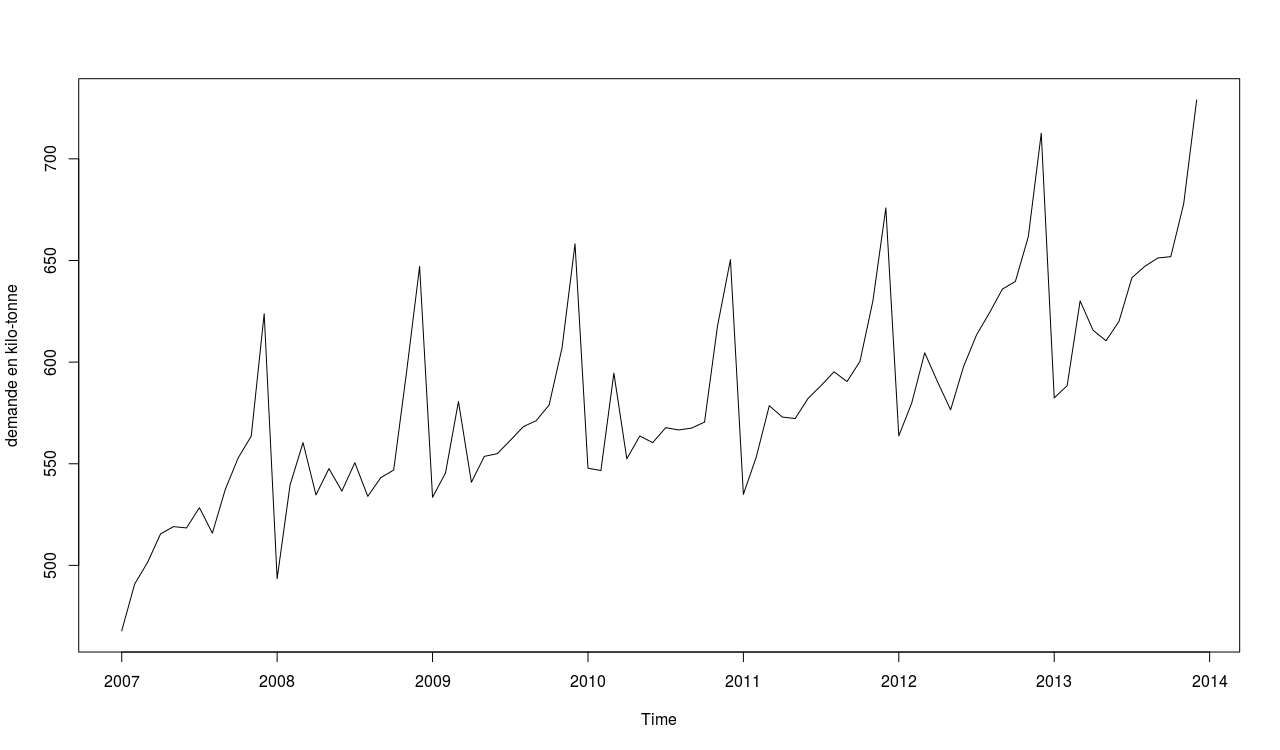
\includegraphics[width=\textwidth]{ch4-images/serie}}
		\caption{Demande en kilo-tonne de fertilisant "Brésil"}
		\label{fig:dem}
	\end{figure}
	\subsection{Décomposition de la série}
	\begin{figure}[H]
		\centering
		\fbox{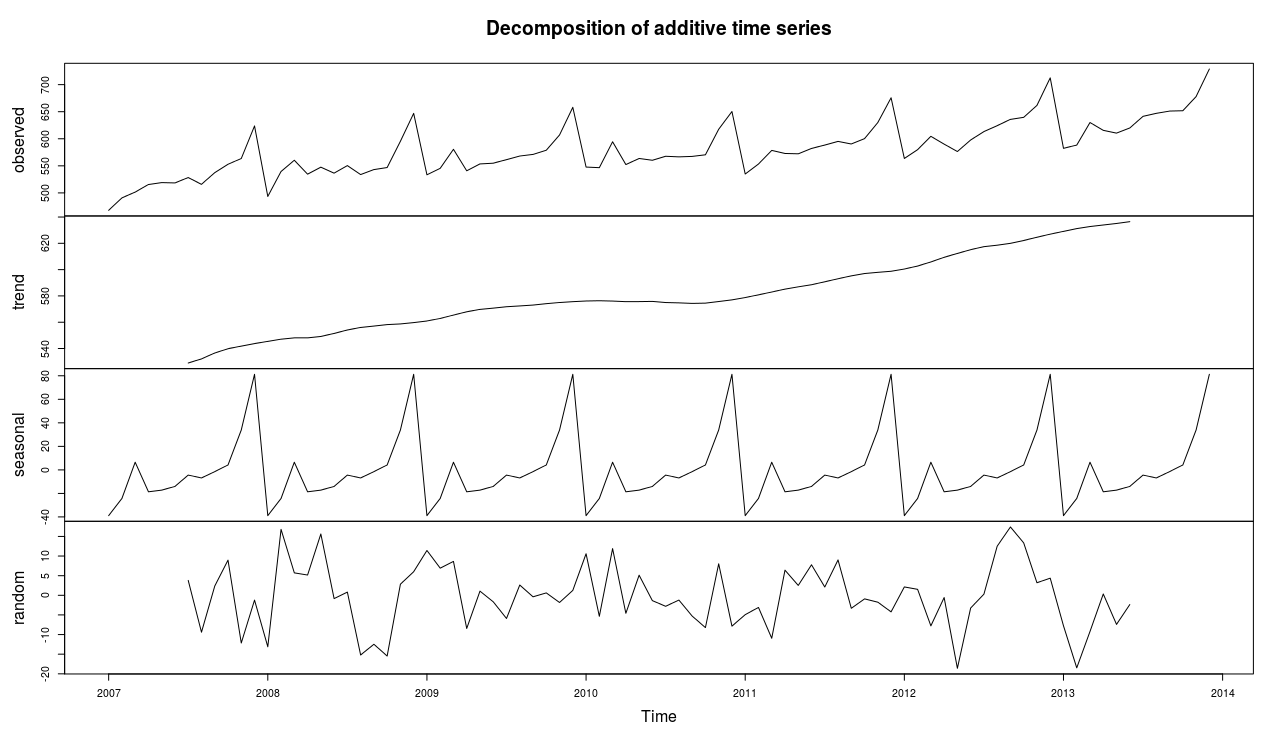
\includegraphics[width=\textwidth]{ch4-images/decomp}}
		\caption{Le tracé de la décomposition "Tendance + saisonnalité + résidu"}
		\label{fig:dec}
	\end{figure}
	La figure ci-dessus montre la série originale (en haut), la tendance estimée (deuxième), la composante saisonnière estimée (troisième) et la composante irrégulière estimée (en bas).On remarque que la tendance est croissante.
	\subsection{Lissage et prévision par la méthode de Holt-Winters}
	\begin{figure}[H]
		\centering
		\fbox{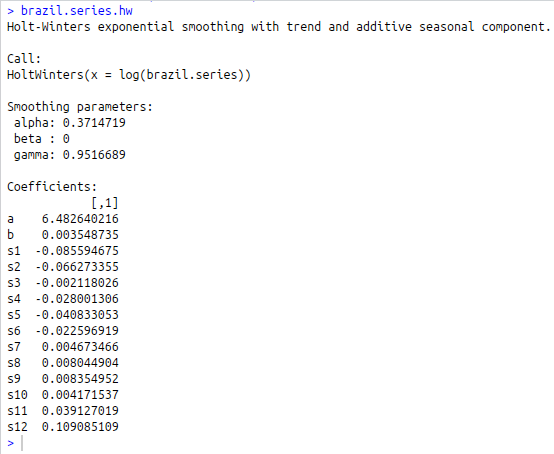
\includegraphics[width=0.5\textwidth]{ch4-images/hw_param}}
		\caption{Paramètre de lissage et coefficients de saisonnalité}
		\label{fig:hw_param}
	\end{figure}
	The estimated values of alpha, beta and gamma are 0.41, 0.00, and 0.96, respectively. The value of alpha (0.41)
is relatively low, indicating that the estimate of the level at the current time point is based upon both recent
observations and some observations in the more distant past. The value of beta is 0.00, indicating that the estimate
of the slope b of the trend component is not updated over the time series, and instead is set equal to its initial value.
This makes good intuitive sense, as the level changes quite a bit over the time series, but the slope b of the trend
component remains roughly the same. In contrast, the value of gamma (0.96) is high, indicating that the estimate
of the seasonal component at the current time point is just based upon very recent observations.
\par
As for simple exponential smoothing and Holt’s exponential smoothing, we can plot the original time series as a
black line, with the forecasted values as a red line on top of that:
	\begin{figure}[H]
		\centering
		\fbox{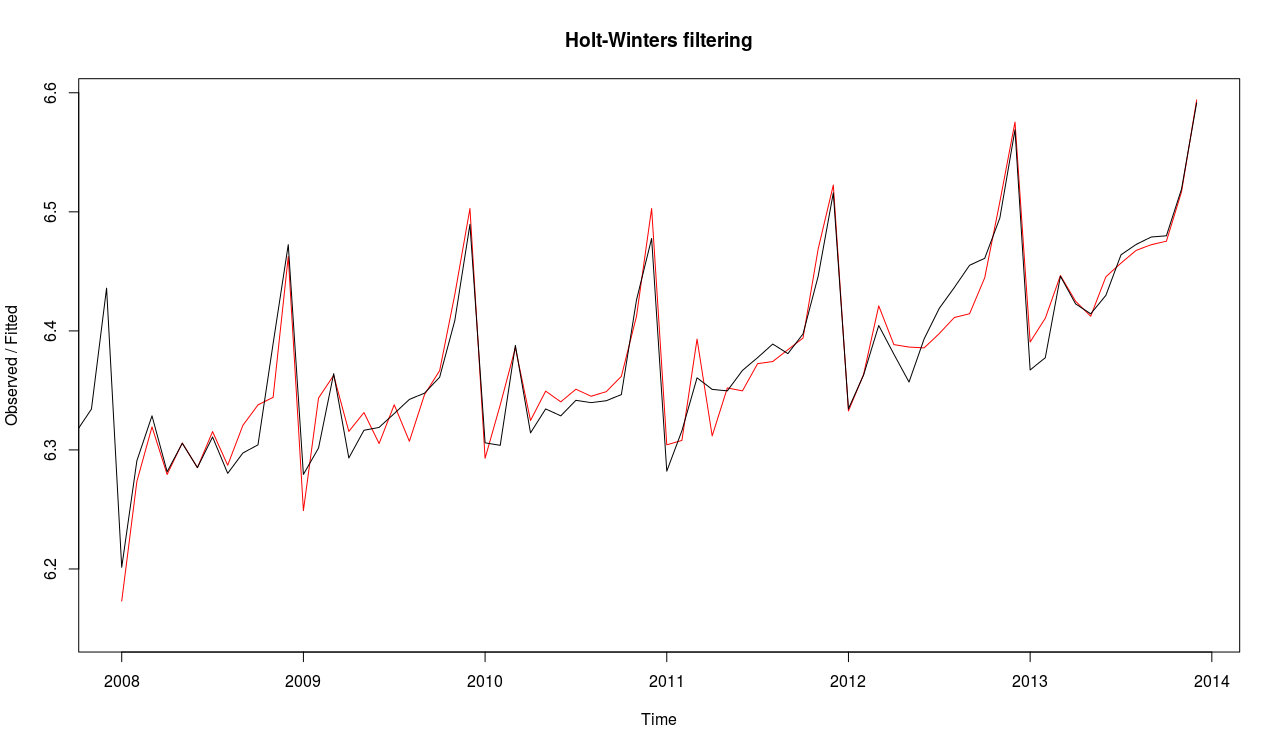
\includegraphics[width=\textwidth]{ch4-images/hw_for}}
		\caption{Courbe estimé par la méthode Holt-Winters.}
		\label{fig:hw_for}
	\end{figure}
	We see from the plot that the Holt-Winters exponential method is very successful in predicting the seasonal peaks.
	
	\begin{figure}[H]
		\centering
		\fbox{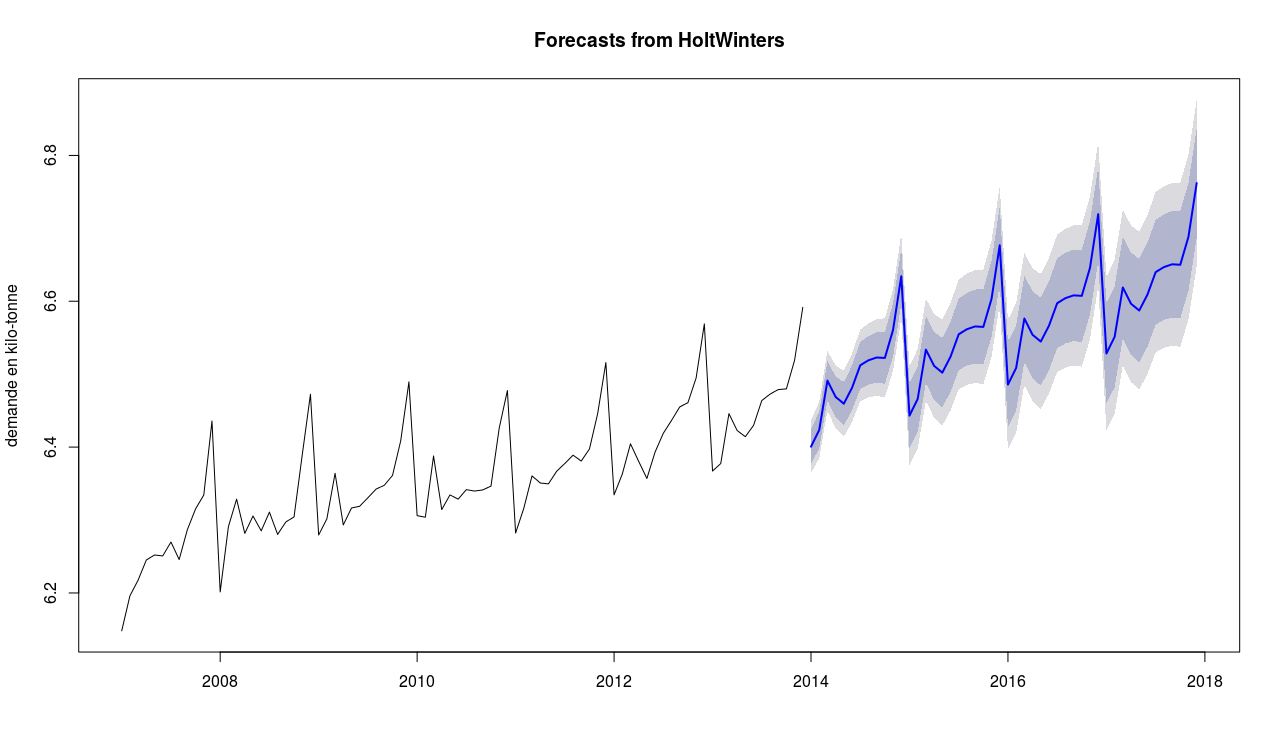
\includegraphics[width=\textwidth]{ch4-images/forcast}}
		\caption{Prédiction pour les quatre ans à venir:}
		\label{fig:forecast}
	\end{figure}
	The forecasts are shown as a blue line, and the orange and yellow shaded areas show 80\% and 95\% prediction
intervals, respectively.

\par
We can investigate whether the predictive model can be improved upon by checking whether the in-sample forecast
errors show non-zero autocorrelations at lags 1-20, by making a correlogram and carrying out the Ljung-Box test:
	\begin{figure}[H]
		\centering
		\fbox{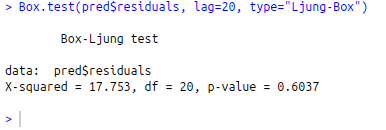
\includegraphics[width=.5\textwidth]{ch4-images/Ljung-Box}}
		\caption{Test de Ljung-Box}
		\label{fig:Q-test}
	\end{figure}
	
	\begin{figure}[H]
		\centering
		\fbox{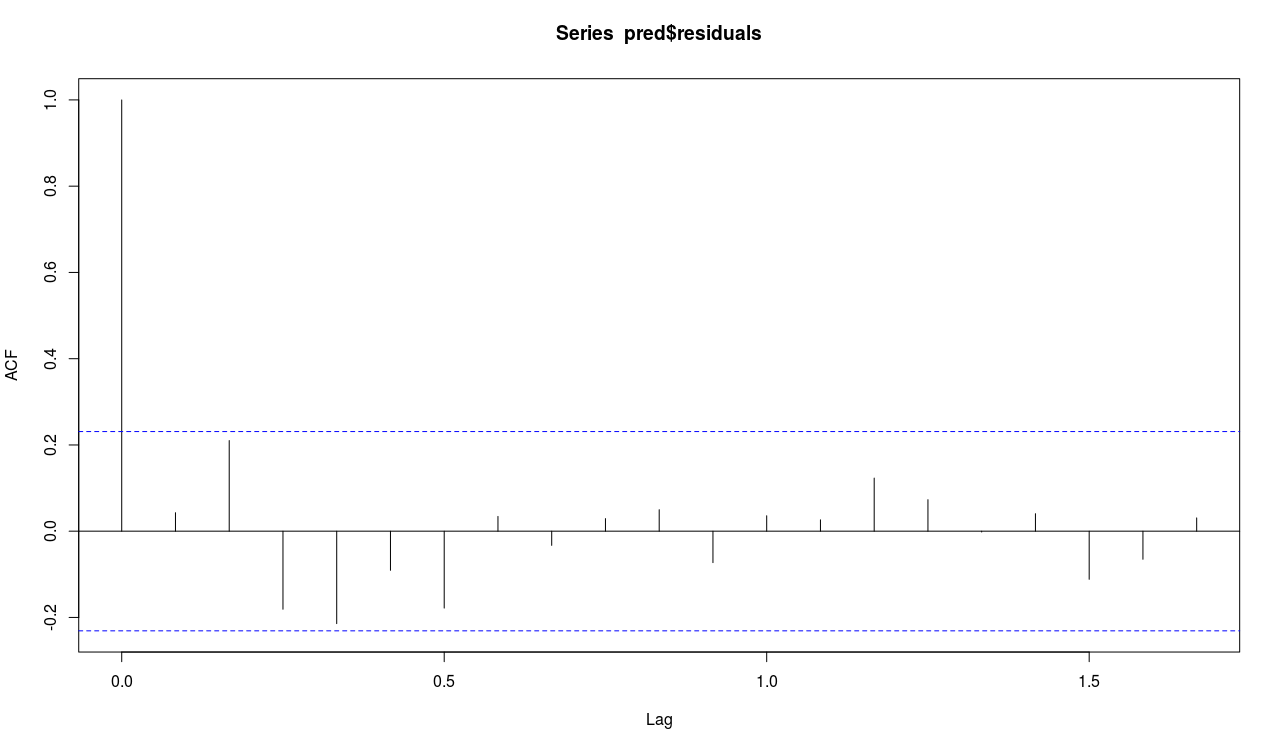
\includegraphics[width=\textwidth]{ch4-images/correlogram}}
		\caption{correlogram}
		\label{fig:correlogram}
	\end{figure}
	
	The correlogram shows that the autocorrelations for the in-sample forecast errors do not exceed the significance
bounds for lags 1-20. Furthermore, the p-value for Ljung-Box test is 0.6, indicating that there is little evidence of
non-zero autocorrelations at lags 1-20.


\par
We can check whether the forecast errors have constant variance over time, and are normally distributed with
mean zero, by making a time plot of the forecast errors and a histogram (with overlaid normal curve):


\begin{figure}[H]
		\centering
		\fbox{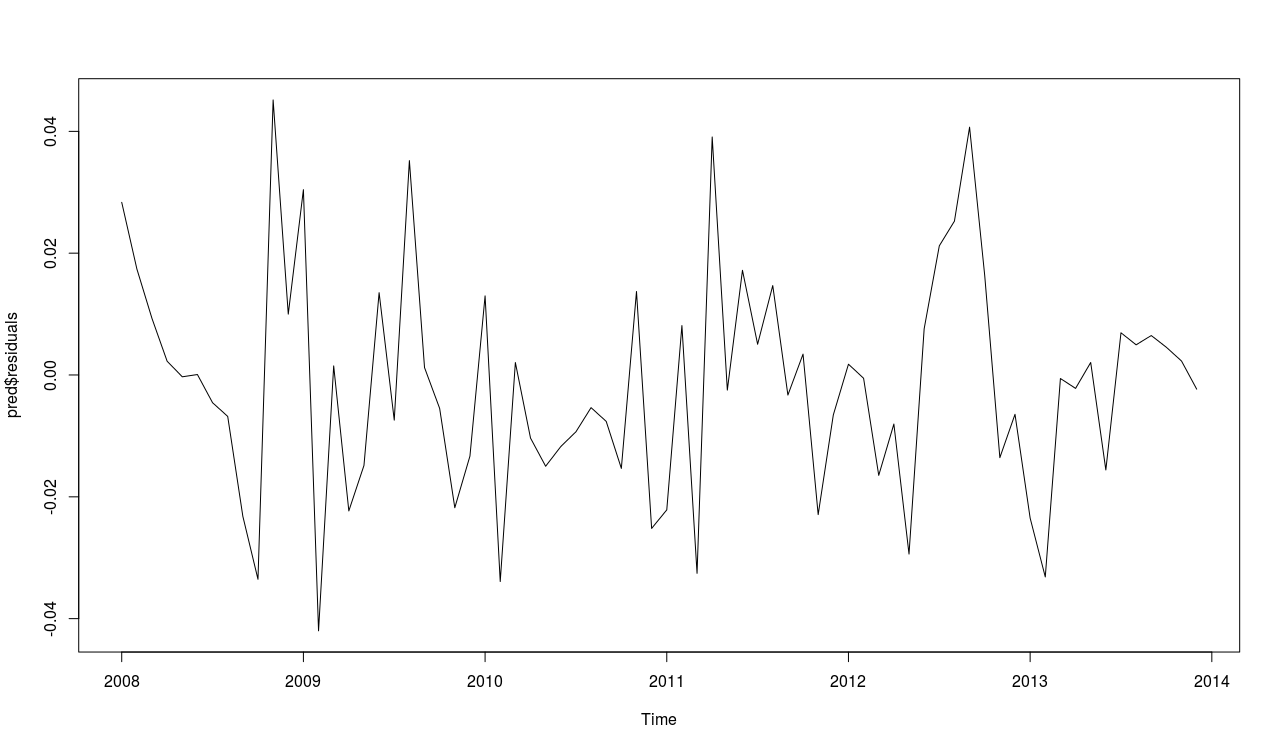
\includegraphics[width=\textwidth]{ch4-images/plot-resi}}
		\caption{Le tracé des résidu}
		\label{fig:plot-resi}
	\end{figure}
	
	\begin{figure}[H]
		\centering
		\fbox{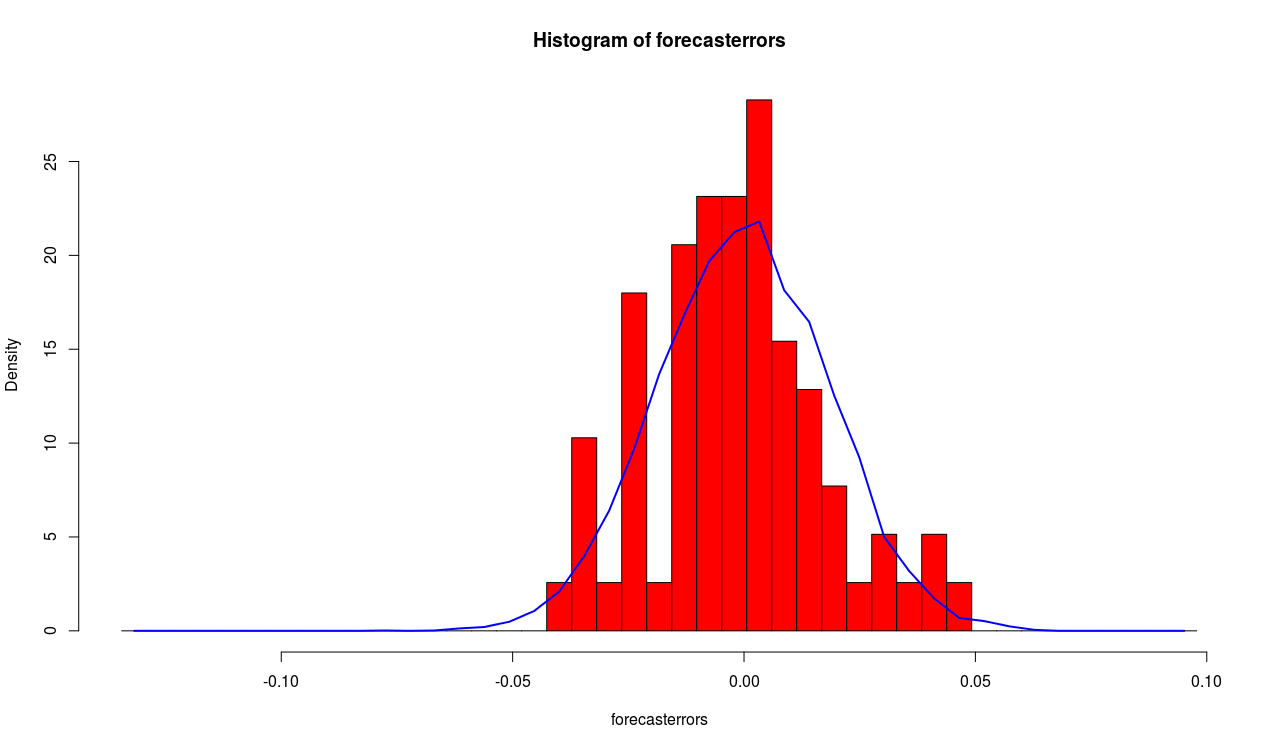
\includegraphics[width=\textwidth]{ch4-images/hist-resi}}
		\caption{Histogramme des résidu}
		\label{fig:hist-resi}
	\end{figure}
	
	
	From the time plot, it appears plausible that the forecast errors have constant variance over time. From the
histogram of forecast errors, it seems plausible that the forecast errors are normally distributed with mean zero.
\par
Thus,there is little evidence of autocorrelation at lags 1-20 for the forecast errors, and the forecast errors appear
to be normally distributed with mean zero and constant variance over time. This suggests that Holt-Winters
exponential smoothing provides an adequate predictive model of the log of sales at the souvenir shop, which
probably cannot be improved upon. Furthermore, the assumptions upon which the prediction intervals were based
are probably valid.